\documentclass{article}
\usepackage{graphicx}
\graphicspath{ {images/} }

\usepackage[english]{babel}
\usepackage[utf8]{inputenc}
\usepackage{indentfirst}

\addtolength{\oddsidemargin}{-.875in}
\addtolength{\evensidemargin}{-.875in}
\addtolength{\textwidth}{1.75in}
\addtolength{\textheight}{1in}

\title{Design 3}
\author{marcinwisniowski1998 }
\date{October 2017}

\begin{document}

\begin{titlepage}
    \centering
	{\scshape\LARGE Truss Design Written Proposal\par}
	\vspace{1cm}
	{\scshape Design III\par}
	\vspace{1cm}
	{\scshape By: Jacob Meiskin, Brendan Shine, and Marcin Wisniowski \par}
	\vfill
	{\scshape November 2017\\Stevens Institute of Technology\\E-231 Section D Group 7\par}
	\vspace{.5cm}
	{\scshape supervised by\\Professor Russo \par}
    \vfill
% Bottom of the page
	{\scshape“I pledge my honor that I have abided by the Stevens Honor System.”}
	\vspace{1cm}
\end{titlepage}

\pagenumbering{roman}
\section{Abstract}
 The following report describes the design, construction, and testing of a single planar truss created in Design III. A truss is a structure composed of slender members joined together at their joints. Joints are commonly formed by bolting or welding each member to a gusset plate. In the real world trusses are frequently used in the construction of roofing and bridges to provide stability to the structures and keep them from breaking apart from heavy load. In many engineering practices, trusses can be found as common bare bones of larger structures. The group three different planar trusses in the Truss Analyzer program, a graphic MATLAB-based software analysis tool, to create a structure strong enough to support the required weight, but also easy enough to construct and recreate in the real world. The comparison of multiple designs lead to a final design that was chosen to be the most rational to our group. After designing the most efficient structure, the design was re-drawn in scale onto a construction template. The truss was constructed with single straight pieces of hollow brass 1/8” square tubing with 0.014” thick walls and soldered together with lead-free solder. After constructing the completed design, the truss was tested using the Truss Buster machine, which applied a single point load at the top-center of the truss. Initially, using the Truss Analyzer, the expected load the structure was expected to withhold was 489.7 pounds of force. In the real test, however, the structure failed at 425 pounds of force through the buckling of a member, not a failure at a joint connection.

\newpage
\tableofcontents
\newpage
\pagenumbering{arabic}


\section{Introduction}
The following report describes the design, construction, and testing of a single planar truss created in Engineering Design III. Engineering Design III focuses on the designing and analysis of structures that are subjected to forces in order to meet real-world requirements. The first few weeks of class were spent testing individual types of forces, including but not limited to tension, compression, bending moment and shear forces onto brass members. For the final project of the E-231, a truss was designed to withstand the most amount of force possible within specific restrictions. Knowledge from previous in-class testing was used in the construction of the plane truss. 


\subsection{Objective}
The objective of this project was to design and build a truss that had the highest predicted failure load, and for that to translate to the actual failure load when the truss was constructed. The truss was designed using the MATLAB-based Truss Analyzer program, which allowed the group to draw a full-scale truss on design paper. The truss design also had to account for a 0.5” gusset plate on each side of the truss to be used as both a holding piece where the Truss Buster lined up and an improvement on the structural capabilities of the truss. During the construction of the truss, solder, flux, a flux brush, a propane torch, and refractory bricks were provided to the group to construct the truss as designed in the program. 

\subsection{Requirements}
The group designed and constructed a plane truss that needed to span an opening of fourteen inches horizontally. Therefore, the bottom members needed to be fifteen inches away to rest on the ends of the Truss Buster for testing. These two support joints needed to be double-gusseted in order to provide stability on the bottom level within the Truss Buster. Similarly, the joint at the top, where the load would be applied also needed to be double gusseted for stability. Due to restrictions with the Truss Buster, the truss design also had a maximum height restriction of four inches from the highest to the lowest point. 

The group was given a total of 84 inches of brass tubing (1/8" square tubing with .014" wall thickness) to create the truss. With these restrictions, the truss design had to be able to hold at least 325 pounds of force applied to the top of the truss, while a goal of more than 475 pounds was set for the group to achieve the maximum amount of points. 


\subsection{Work Breakdown}
The project presented to the group led the group to designate team roles to each person within the group, in order to deal with each section of the project. The team roles broke down into three distinct jobs: design, construction, and documentation. The group used a work breakdown structure as a base to delegate what each team member needed to do to complete the project as efficiently as possible. The design portion of the group required designing the trusses and deciding which truss was the most effective for the given objective. The construction required cutting materials and creating the truss that was chosen. The documentation portion had to create the time and job management charts, and create the truss on the design paper.

\newpage

\begin{figure}[ht]
\caption{Work Breakdown Structure}
\centering
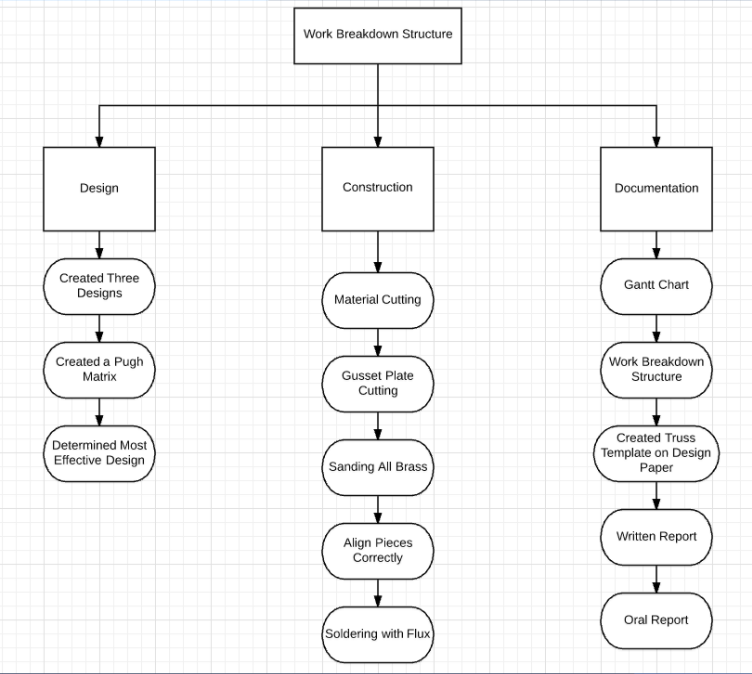
\includegraphics[width=400pt]{WorkBreakdown.png}
\end{figure}

\subsection{Gantt Chart}
The group was also led to create a Gantt chart in order to manage the time allotted. The group was presented with a lot of work that had to be completed, and despite a team role given to each member, in most cases the entire team worked on tasks together to complete the tasks as quickly as possible. The construction of the truss was the most time consuming piece of the project, as seen in the task breakdown. The group was able to stay on pace with the tasks as originally designed, and the truss was completed as projected with time to spare.

\begin{figure}[ht]
\caption{Gantt Chart}
\centering
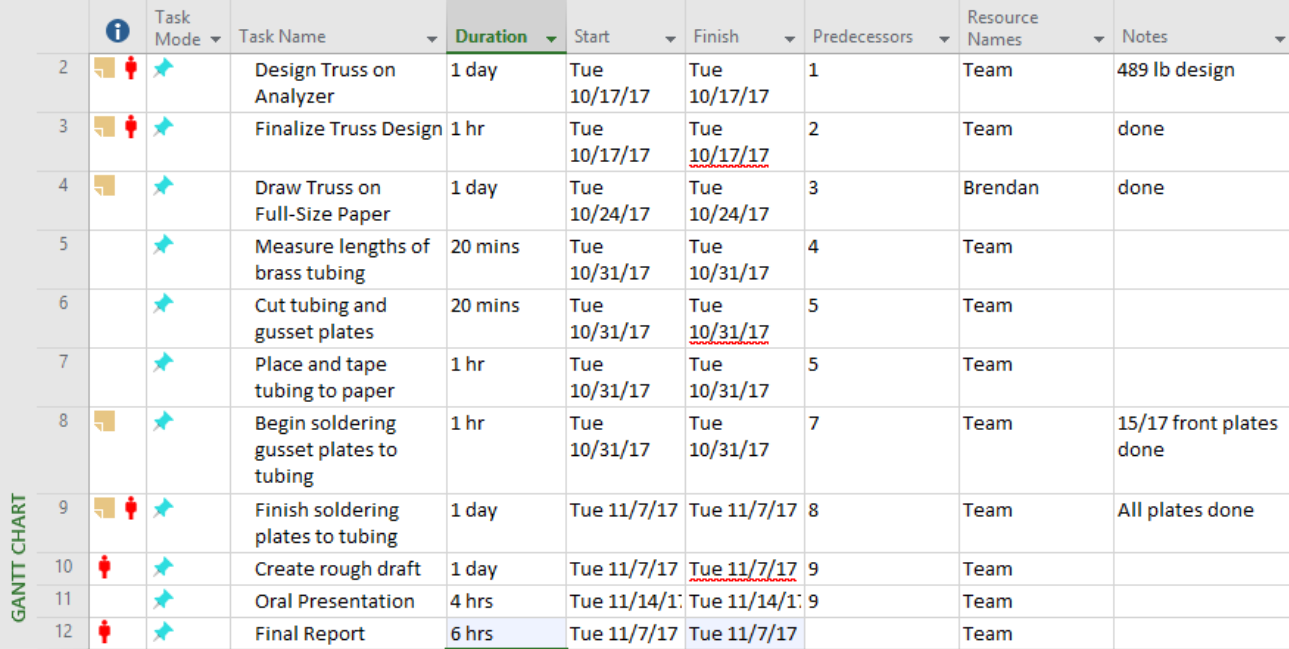
\includegraphics[width=400pt]{GanttChart.png}
\end{figure}

\newpage

\section{Discussion}
The group spent most of its time creating designs and analyzing them. By using the added benefits of the Truss Analyzer Program, the Buckling Analysis Formula Solver, and a period of time to learn how to correctly solder members together, the group was able to create the most optimal truss of the ones envisioned by the group. Within the next few subsections, the design process is explained thoroughly to lead the reader across the overall design challenges and solutions. 


\subsection{Truss Analyzer}
 One of the biggest technical challenges was creating a truss design that fit within the specified restrictions, while also being able to support a large enough load. The group initially began to design trusses individually within the Truss Analyzer program. The program allowed us to quickly develop working designs without the need of many math calculations or the building and testing of prototypes. The use of a pre-made program sped up the ability to design multiple trusses to compare with each other. 
 
\begin{figure}[ht]
\caption{Truss Analyzer Program}
\centering
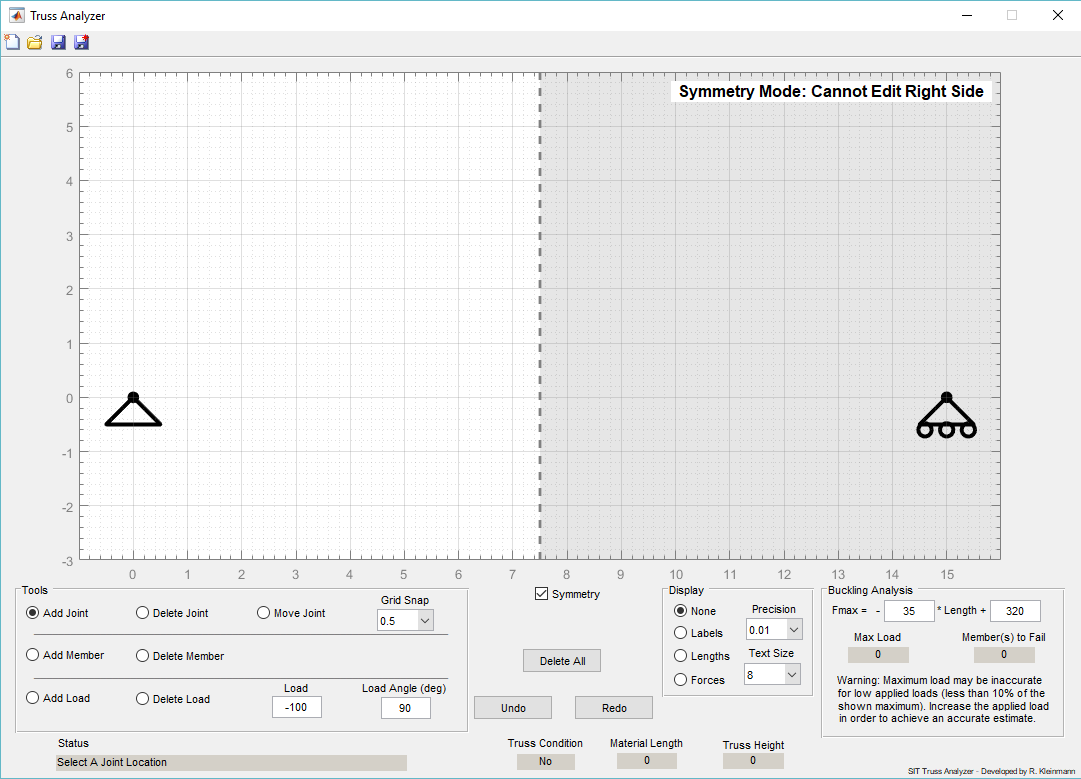
\includegraphics[width=400pt]{TrussAnalyzerProgram.png}
\end{figure}

\newpage

 By using the Buckling Analysis program in the bottom right of the Truss Analyzer each group member was able to quickly compare multiple trusses based on theoretical loads in order to create the strongest truss design. From previous experiments within the lab, the buckling analysis formula was estimated between multiple groups to be given below. The group used this formula to correctly assess the maximum strength each design could withhold without failing and ranked designs according to their maximum load. Similarly, since the buckling analysis worked in real-time, the group was able to use trial and error by moving joints around to see how the values changed on the overall structure. Thanks to this program, the design process was much easier than working out the mathematical equations each time a change to a truss was made and it greatly sped up the process of testing different shapes and using trial and error to find the best truss design. 

\begin{figure}[ht]
\caption{Buckling Analysis Formula}
\centering
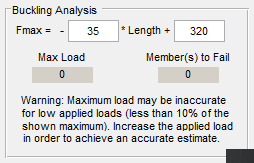
\includegraphics[width=200pt]{BucklingAnalysis.png}
\end{figure}


\subsection{Design Section}
For the first week, the group worked on planning out how to create the strongest truss design within the Truss Analyzer program. After trying multiple test designs, the group realized that trusses in football, or egg shaped patterns seemed to hold a larger force than other truss designs that the group tried to do. After realizing this fact, the group began to work to optimize the better truss designs until multiple ones could hold a large load. 

\subsubsection{Pugh Matrix}
Three final designs were created, one by each member, to be further assessed for multiple factors of complexity and strength. Therefore, the team turned to creating a Pugh Matrix in order to feasibly compare the models under specific conditions. Below are each of the three designs, along with the Pugh Matrix comparing each one. 

\begin{figure}[h]
\caption{Conceptual Design 3}
\centering
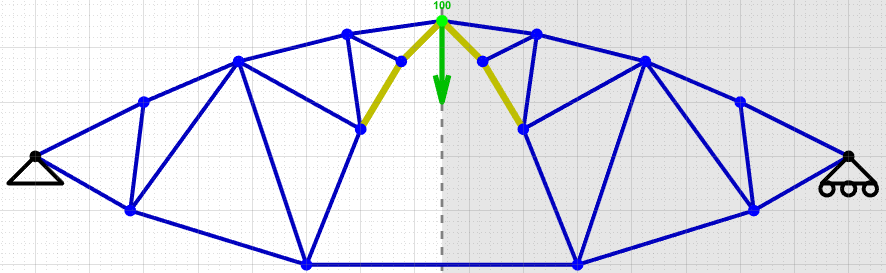
\includegraphics[width=400pt]{truss449.png}
\end{figure}

Initially, the group's first truss over the strength of 400 lbs of force can be seen in Figure 1 above. The football shaped curves on the outer truss edges were very apparent and the joint were made to allow for a stronger resemblance to this shape. This design was the first to incorporate a drooping bottom curve, which stayed within the other designs. However, the large sag created problems with keeping the end supports flat, in order for it to rest well on the Truss Buster machine, and the overall strength was based on its height, which was taller than the allowed specifications. When the group tried to shrink the truss size down, the strength significantly dropped.


\begin{figure}[ht]
\caption{Conceptual Design 1}
\centering
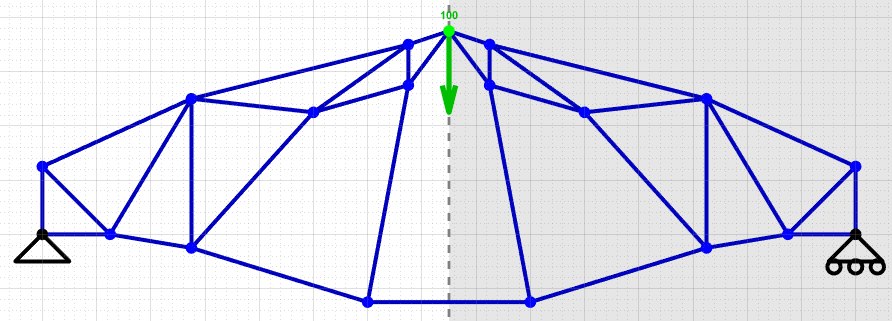
\includegraphics[width=400pt]{truss552.png}
\end{figure}

This second design incorporated a different sagging technique, by making it curve the opposite direction on the bottom edge. While the first was a generic, positive parabola throughout, this design actually curved in the opposite direction until it met in the center for a straight edge. While this design was the strongest that was created by the group, it was also the most complex, using the most material the most members, and the most joints. While testing within the program, the group also noticed that even slight changes in the angles of some joints led to very sharp decreases in its strength, so while it was the strongest, it was similarly the most unstable. 

\begin{figure}[ht]
\caption{Conceptual Design 2}
\centering
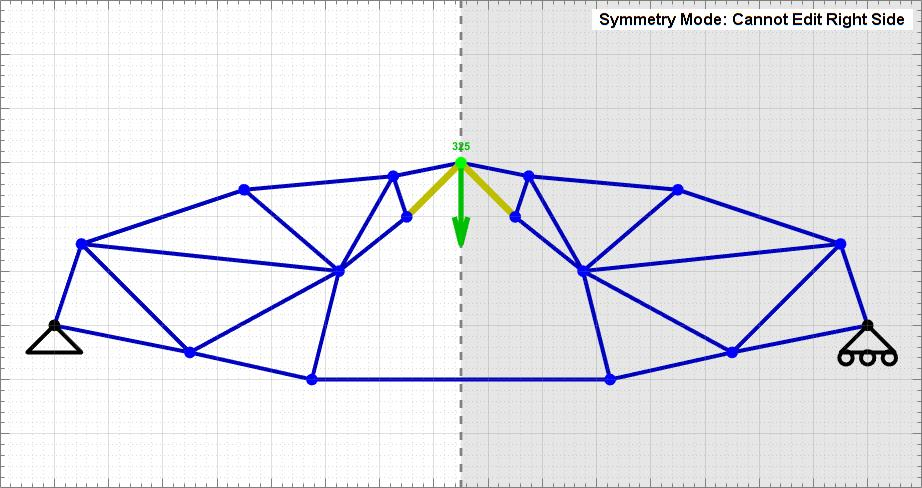
\includegraphics[width=400pt]{truss489.jpg}
\end{figure}

The third conceptual design was made unlike the others, with an almost horizontal member connection two joints. While this truss design still started off around the initial egg-shaped design that the other two did, it slowly deviated away to become far more rectangular than the other two designs, which both had large droops in their designs. While this design was weaker than the second conceptual design, the group ended up choosing this one for multiple reasons. First, while still relatively strong, this truss design was the only one that completely fit within the guidelines of the build. The other two trusses would need to be modified to fit within the height restrictions, mostly because of their football-shaped strength. Similarly, the truss designed felt like a strong middle group between the quite simple design of Conceptual Design 3, and the quite strong design of Conceptual Design 1. 

The Pugh Matrix created also followed the same trends that the group initially saw in the design and gave it the highest score of the three, confirming our personal choice to choose this truss design to build. 

\begin{figure}[ht]
\caption{Pugh Matrix}
\centering
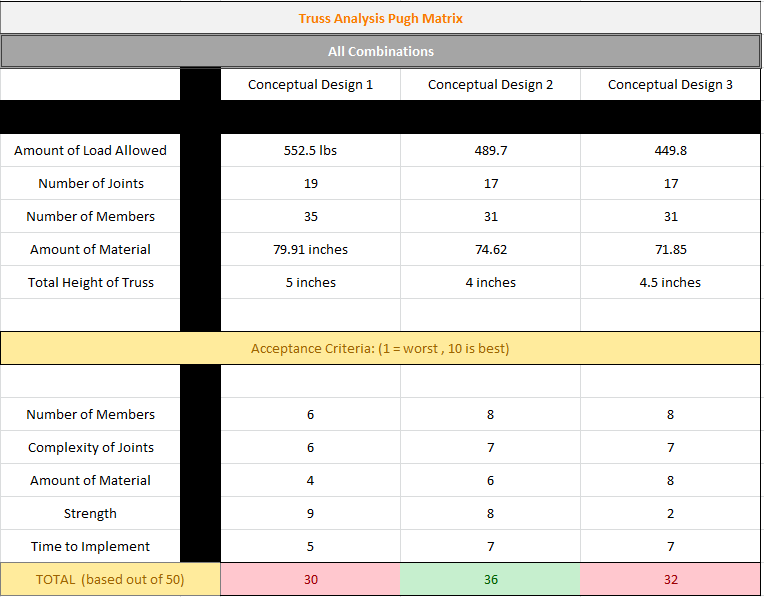
\includegraphics[width=\textwidth]{PughMatrix.png}
\end{figure}

\newpage

Similarly, it was important for the group to look at the excel data for each of the truss designs and learn from the values recorded. Overall, the group was able to create a strong truss by staying away from zero force members, and similarly distributing the load evenly across the members that it had. When looking at the designs, many of the forces are approximately the same size across each of the members used within the design. For instance, in the first conceptual design, the forces strongly stay within the limits of approximately -55 to 55 pounds of force with very few outliers. Finally, the group used a long member in tension at the bottom of each design to keep the designs sturdy, as compression causes buckling but tension does not, and less complex. 

\begin{figure}[ht]
\caption{Excel Data}
\centering
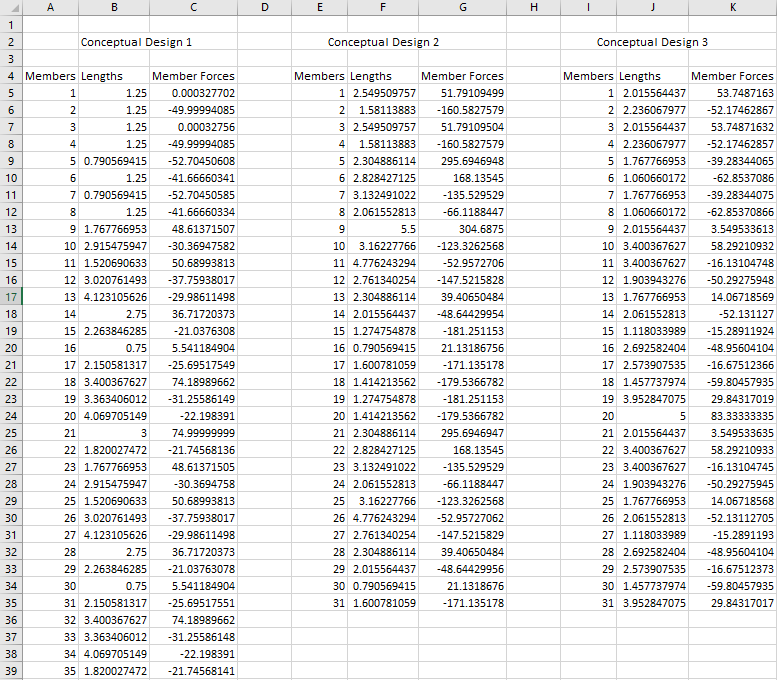
\includegraphics[width=450pt]{TrussExcel.png}
\end{figure}

\newpage

\subsubsection{Chosen Design}
The group agreed that the second conceptual design was the strongest design made in the Truss Analyzer program and began to evaluate its strong and weak points. Based on the Truss Analyzer program, the design had a strong balance of members in tension and compression without any members being zero force members, allowing for a load distribution across each of the members. In the design, the failing members appeared directly below the load application. While initially the group tried to alter the design around this area to gain more load capacity, the amount of extra complexity created was not worth the minimal load capacity added to the design strength. In the end, the chosen design was predicted to hold 489.7 pounds of force and fail on members 18 and 20 near the application of the load force. Also, the design chosen was made up of 31 members and 17 joints, being relatively simple to design. Finally, only 74.62 inches of brass material was used, of the overall 82 inches provided which allowed the group to receive a stronger score per weight of the design. 

\begin{figure}[ht]
\caption{Truss Values}
\centering
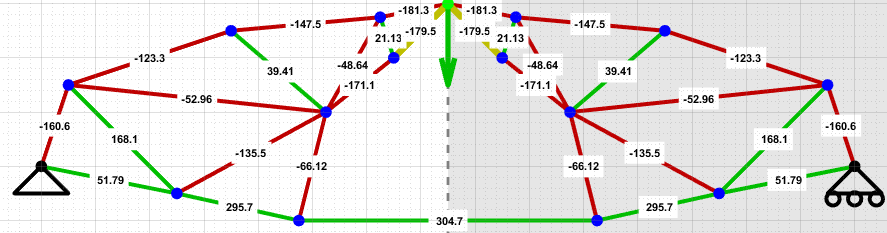
\includegraphics[width=400pt]{TrussDesignWithValues.png}
\end{figure}

\subsection{Fabrication}
After creating and analyzing the group's design from the Truss Analyzer program, the group went on to build the truss with the use of square brass tubing, brass gusset plates and lead-free solder. Below is a list of materials used in the construction of the truss design. The brass tubing used was a hollow brass 1/8" square (outside dimension) with 0.014" wall thickness. 

\begin{figure}[ht]
\caption{Construction Materials}
\centering
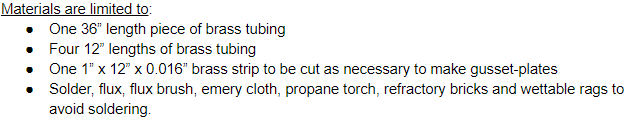
\includegraphics[width=300pt]{ConstructionMaterials.png}
\end{figure}

\subsubsection{Full-Scale Design}
In order to create an accurate depiction of the design created in the Truss Analyzer program, the truss was recreated in full-scale on Design Paper. The scale drawing helped to assure that members would be cut correctly and would be the correct length. The drawing also allowed the group to tape the members into the correct place to verify that all parts fit together at the correct angles. 

\subsubsection{Cutting Members}
Each member was cut to size using a band saw with a cutting blade of 1/16". Fortunately, since the group had a lot of extra material this loss of material due to the cutting blade was not an issue when creating the full-scale model. Since the brass tubing was given in lengths of 12" and one in a length of 36", the group decided to emphasize a notching technique into the construction of the truss. By notching and then bending the material into the angles, instead of completely cutting through the material, the truss was able to stay stronger at those joints. Likewise, the notching technique allowed many joints to stay more rigid, and therefore easier to solder into the correct angles than those that were cut through entirely. Below is an image of the fully cut and assembled truss design in full-scale. 

\begin{figure}[ht]
\caption{Design Paper}
\centering
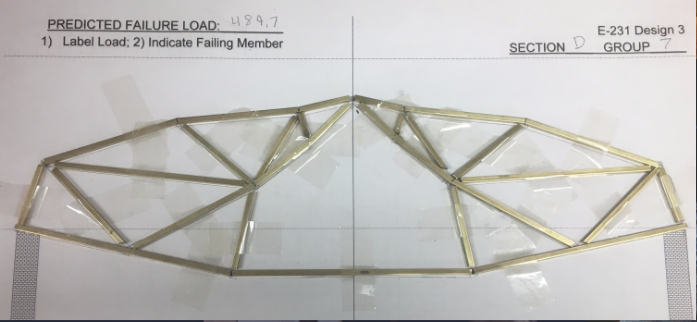
\includegraphics[width=400pt]{DesignPaper.png}
\end{figure}

\newpage

\subsubsection{Soldering}
Before soldering, the group confirmed that the cut members fit correctly onto the full-scaled design and tapes each of the pieces down. In order to keep the angles as accurate as possible, the group decided that the design would stay taped down to the design paper and be soldered while still attached to the paper. While this ended up burning up the paper in the end, each member was much easier to hold in place and solder, creating a very accurate design. 

\subsubsection{Joint Connections}
Each brass member and gusset plate was sanded down to remove blemishes and then coated in flux to allow the solder to flow and fill in any spaces under the members. Then, while one member melted the solder, the other members pressed the members down into the gusset plate to create a strong connection. The group decided to start with easier joints and work their way up to the more complex five and six-member joints. This was in order to lower the amount of members that needed to be pushed down into the gusset plate and lower the chance of a member shifting out of position. Likewise, by starting at easier joints and moving up, the group was able to lower the chances of annealing which occurs due to an excessive application of heat onto the brass. Each joint was efficiently soldered, leading our design to not fail due to a joint, but instead due to a member failure. Below is an image of our completed truss model:

\begin{figure}[ht]
\caption{Completed Truss}
\centering
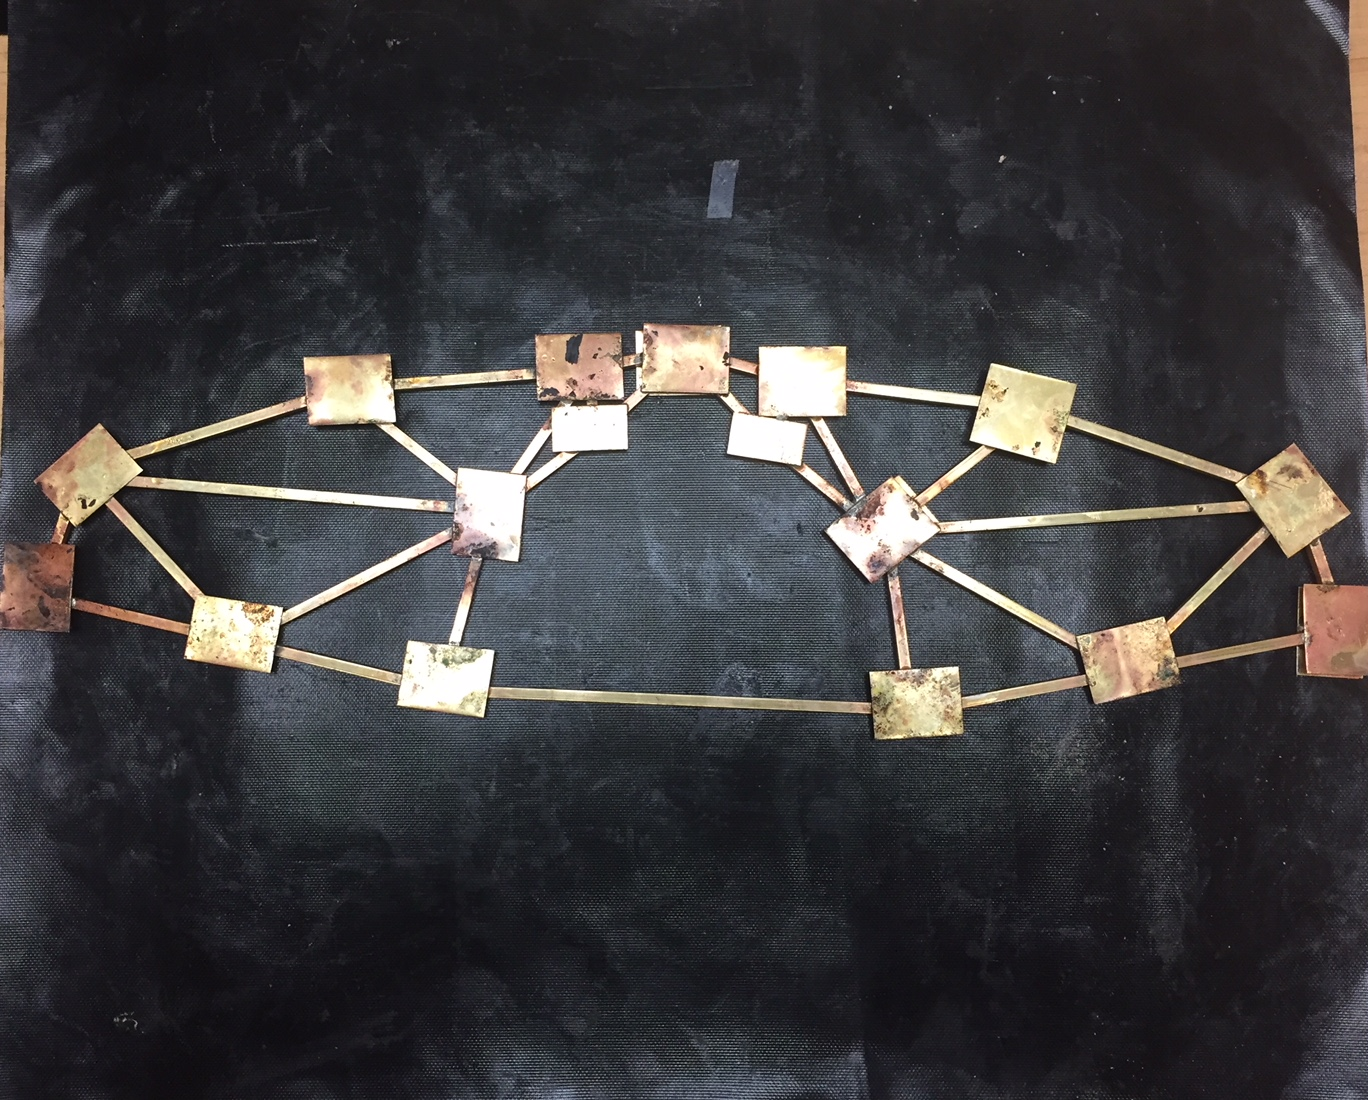
\includegraphics[width=400pt]{BrassTruss.jpg}
\end{figure}

\newpage

\subsection{Testing}
\subsubsection{Truss Buster}
After construction was completed, the truss was tested for maximum load capacity within the Truss Buster. Using the Truss Buster, a single point load was applied to the truss at the top-center of the structure. The side plates (one transparent) of a test fixture provided lateral stability for the Truss Buster. The span will be defined by the distance between two plywood "support blocks" which will provide a 1" height for elevated trusses. Below is an image of the Truss Buster:

\begin{figure}[ht]
\caption{Truss Buster}
\centering
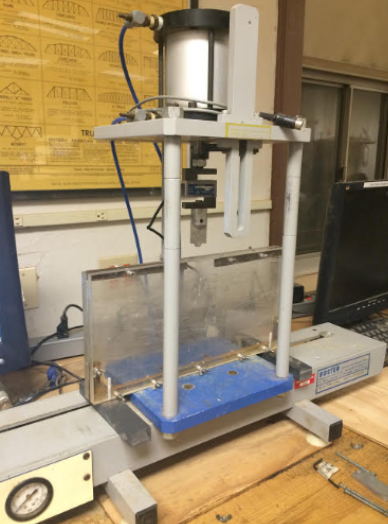
\includegraphics[width=300pt]{TrussBuster.png}
\end{figure}

\newpage

\subsubsection{Results}
The design truss ended up withstanding 425 pounds of force before buckling at one of its outside members. This ended up being the second highest force within the entire section, even while being predicted to be the fourth highest. This only comes back positively towards the group, showing that either the group's workmanship was better than other groups or the design was less complex, while just as strong. 

Other values calculated include, actual to predicted load percent error and actual load to weight ratio. For both of these values, the group ended up scoring above average in the section being the third lowest error, and the fourth highest load to weight ratio out of eight groups. 

\begin{figure}[ht]
\caption{Results}
\centering
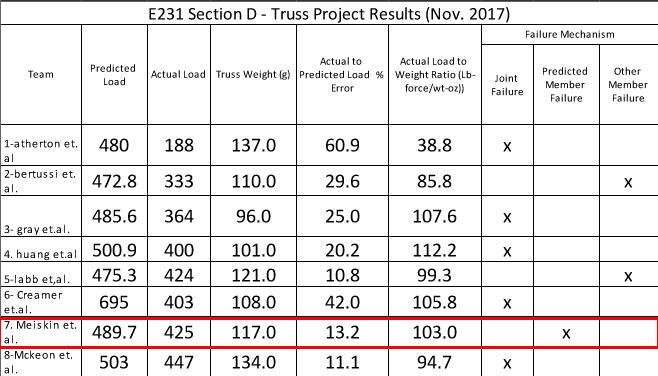
\includegraphics[width=400pt]{TrussResults.png}
\end{figure}



\newpage

\section{Conclusions and Recommendations}
Group 7 placed second in the competition with the truss designed. All of the requirements were met, and the truss was projected to hold a maximum of 489.7 pounds. However, when the group tested the truss, there was a failure at member 3, resulting in the truss only being able to support 425 pounds. There was a small percent error of 13.2, which was relatively low compared to the rest of the section’s percent errors. There was also a load to weight ratio of 103 lb/oz, which was one of the lowest load to weight ratios among all of the groups competing. The weakest member projected was not the one that was identified when testing the truss, so we believe that there was a small error when placing the truss on the lifts when testing the truss. The group knew that if any of the angles were changed between the members and the joints were not sufficiently soldered, then the truss would have broke at a much smaller load than what it experimentally did. 

\begin{figure}[ht]
\caption{Truss Failure}
\centering
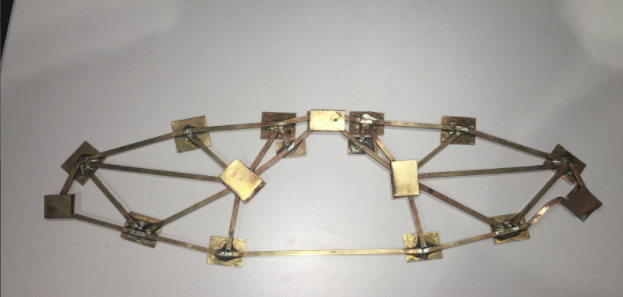
\includegraphics[width=350pt]{BuckledTruss.png}
\end{figure}

\subsection{Testing Failure}
Interestingly, the member that failed for the group was not the one that was predicted to fail. Under further inspection, the member wasn't even one that should have failed under any circumstance, since it was under a small amount of tension, not compression. Therefore, the buckling was not made by the load applied at the center of the truss, but through a different pressure point. The group believes, that as the truss was put under more and more force, the supports it was resting on moved in from under it. As the support moved in, it began to rest on the length of the bottom member itself and therefore created a resultant force back into it from below, forcing it to buckle inwards. If caught beforehand, the truss would have withheld an even higher force, maybe even making it the strongest in the section.

\begin{figure}[ht]
\caption{Joint Failure}
\centering
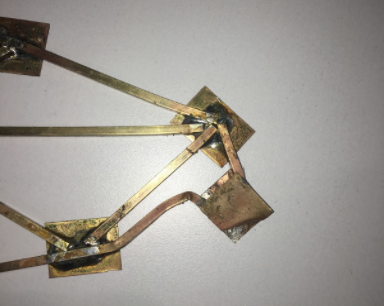
\includegraphics[width=300pt]{BuckledMember.png}
\end{figure}

\subsection{Recommendations}
Due to the very small percent error, there is not much that the group would change to the truss to create a better outcome. However, if given the opportunity, the group would have spent more time soldering at the easier joints and then worked its way up to making the harder solders. With this mentality, the group would start with a basic design for the truss and then work up to the fine details in which the truss could successfully hold all of the desired load. Another recommendation that could have helped improve the truss was by creating horizontal connections at the endpoints of the truss. As previously mentioned, the group believes the testing failure occurred because of angled gusset plates causing the truss to slowly slide away from its initial placement and onto the member at the bottom of the truss. The group believes that the bending of member 3 happened due to this, after enough load was added to the truss. By altering the design of the truss so that there was a small section of completely horizontal members at the ends to be able to rest the truss on, the truss could have supported more weight in the end. 

\subsection{Conclusions}
Overall, this project was very successful. With a small percent error and a small load to weight ratio, Group 7 believes that not much can be changed to the truss design to improve it. Some of the key successes that helped the group be so successful when testing the load were staying very accurate when creating the angles between the members and having solid soldering foundations at the joints connecting the members. The failure experienced was due to having angled gusset plates at the endpoints, causing the supports to slide off the plates and onto the member itself and creating a point of pressure for the member to bend at. 

\newpage
\setcounter{page}{1}
\renewcommand{\thepage}{A-\arabic{page}}
\section{Appendix: Figures and Tables}

\subsection{Figure 1: Work Breakdown Structure}
\begin{center}{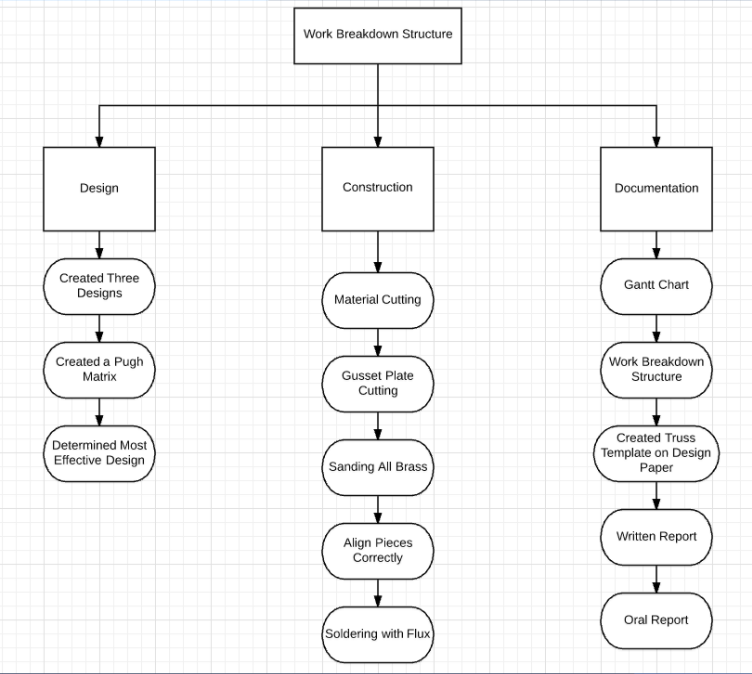
\includegraphics[height=8cm]{WorkBreakdown.png}}\end{center}

\subsection{Figure 2: Gantt Chart}
\begin{center}{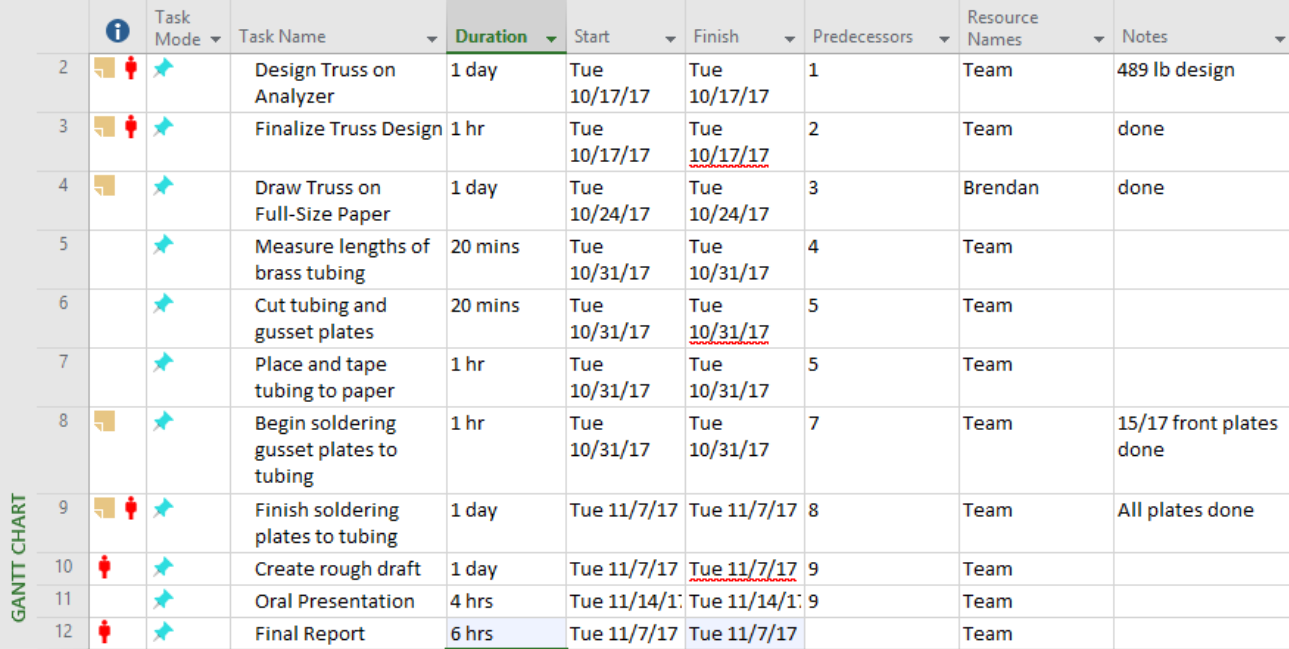
\includegraphics[height=8cm]{GanttChart.png}}\end{center}

\subsection{Figure 3: Truss Analyzer}
\begin{center}{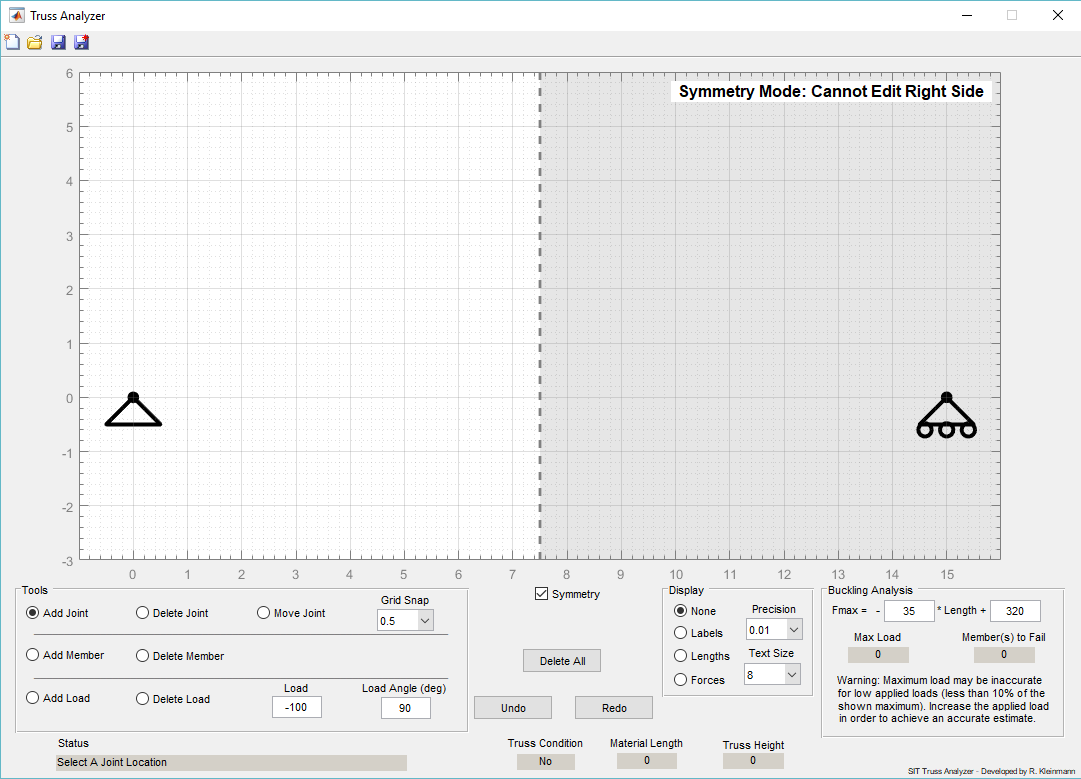
\includegraphics[height=8cm]{TrussAnalyzerProgram.png}}\end{center}

\subsection{Figure 4: Buckling Analysis Formula}
\begin{center}{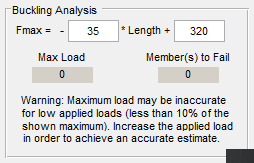
\includegraphics[height=5cm]{BucklingAnalysis.png}}\end{center}

\newpage
\subsection{Figure 5: Conceptual Design 3}
\begin{center}{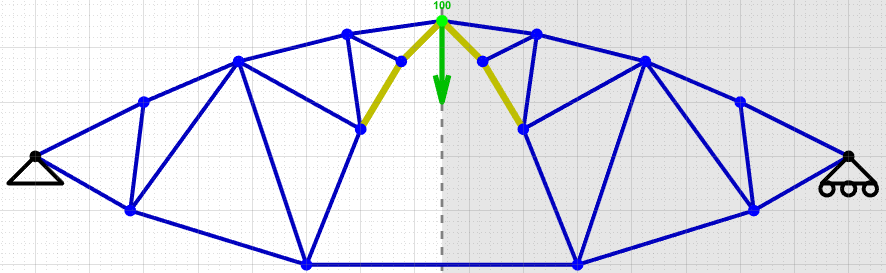
\includegraphics[height=4cm]{truss449.png}}\end{center}

\subsection{Figure 6: Conceptual Design 1}
\begin{center}{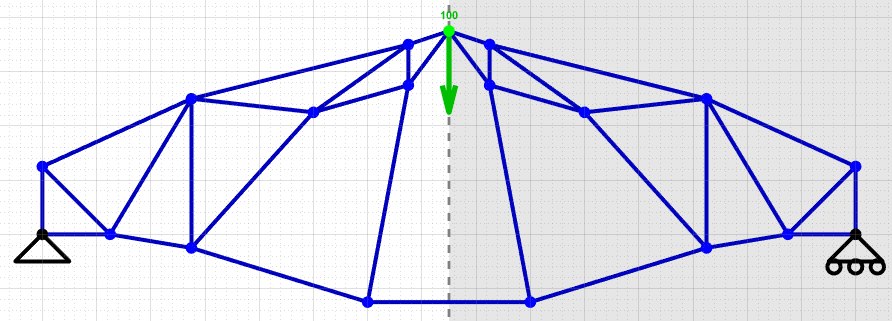
\includegraphics[height=4cm]{truss552.png}}\end{center}

\subsection{Figure 7: Conceptual Design 2}
\begin{center}{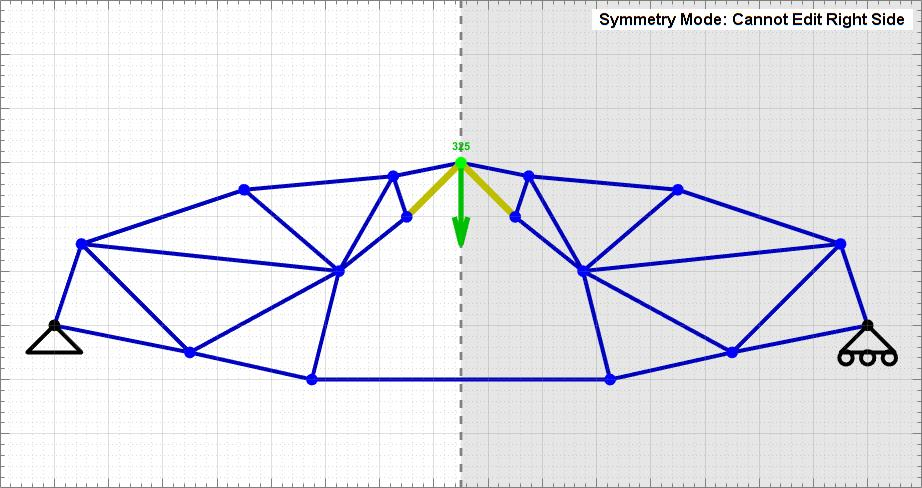
\includegraphics[height=8cm]{truss489.jpg}}\end{center}

\subsection{Figure 8: Pugh Matrix}
\begin{center}{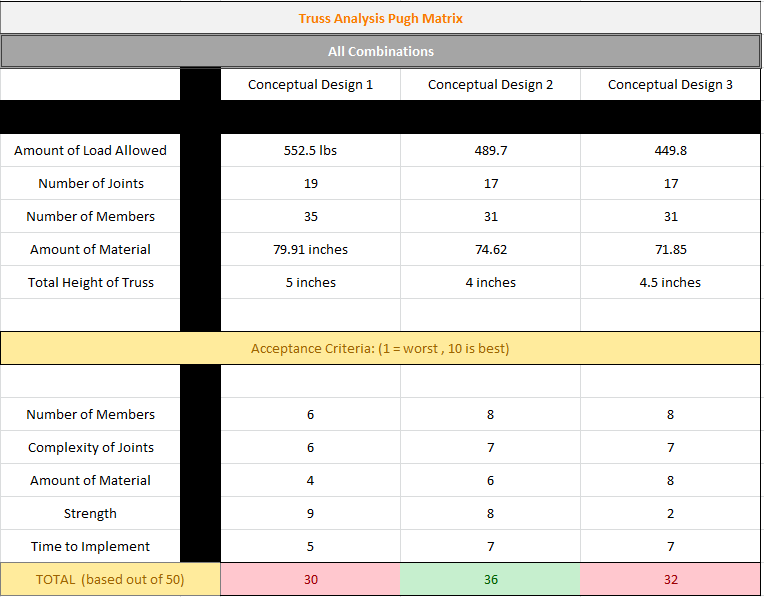
\includegraphics[height=8cm]{PughMatrix.png}}\end{center}

\subsection{Figure 9: Excel Data}
\begin{center}{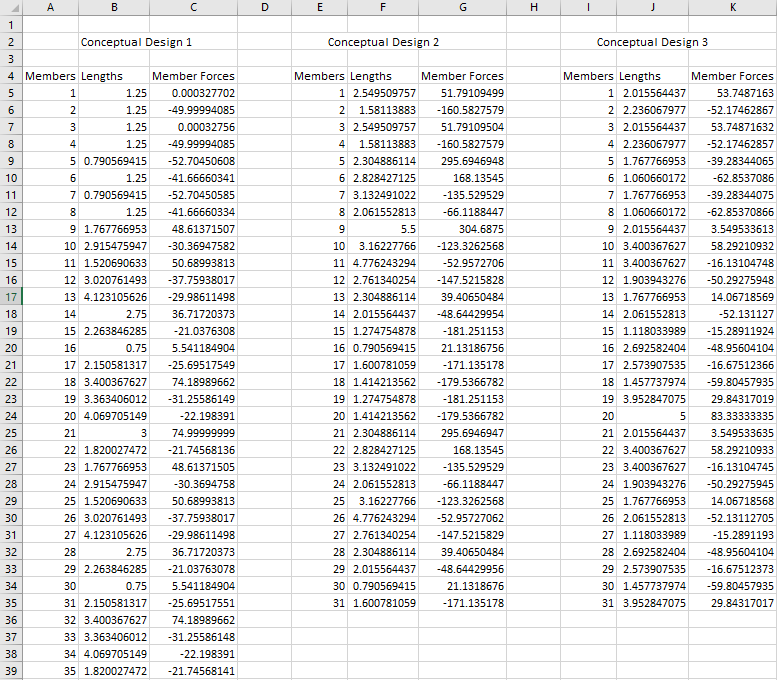
\includegraphics[height=11cm]{TrussExcel.png}}\end{center}

\subsection{Figure 10: Chosen Truss}
\begin{center}{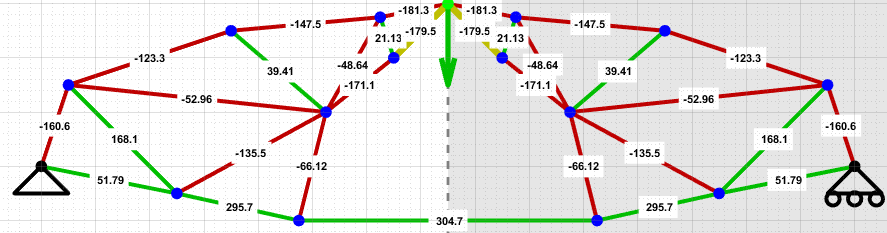
\includegraphics[height=4cm]{TrussDesignWithValues.png}}\end{center}

\subsection{Figure 11: Construction Materials}
\begin{center}{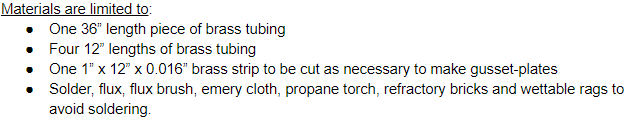
\includegraphics[height=3cm]{ConstructionMaterials.png}}\end{center}

\subsection{Figure 12: Design Paper}
\begin{center}{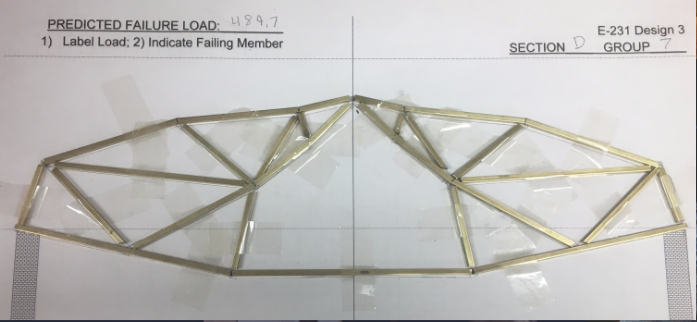
\includegraphics[height=8cm]{DesignPaper.png}}\end{center}

\subsection{Figure 13: Completed Truss}
\begin{center}{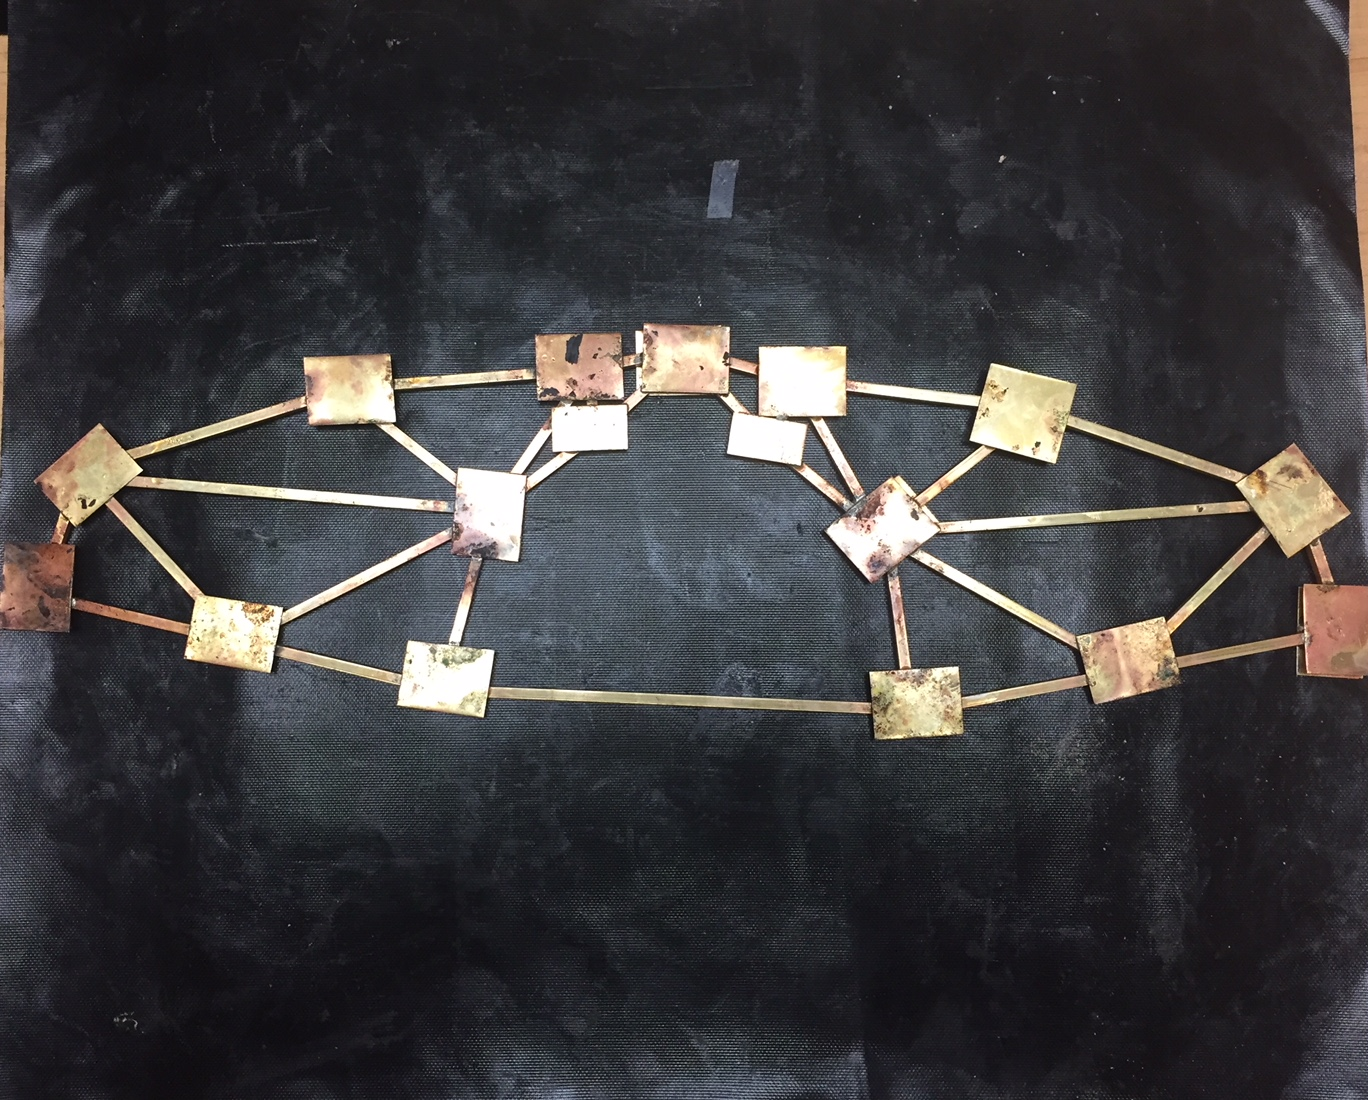
\includegraphics[height=8cm]{BrassTruss.jpg}}\end{center}

\subsection{Figure 14: Truss Buster}
\begin{center}{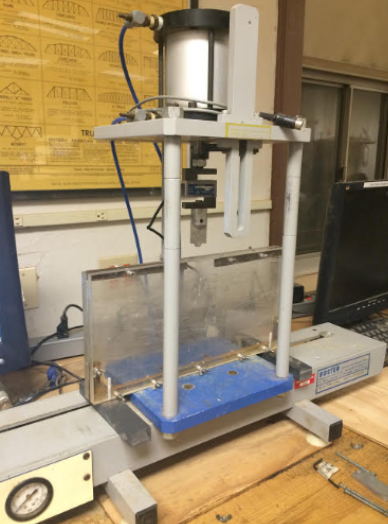
\includegraphics[height=8cm]{TrussBuster.png}}\end{center}

\subsection{Figure 15: Section Results}
\begin{center}{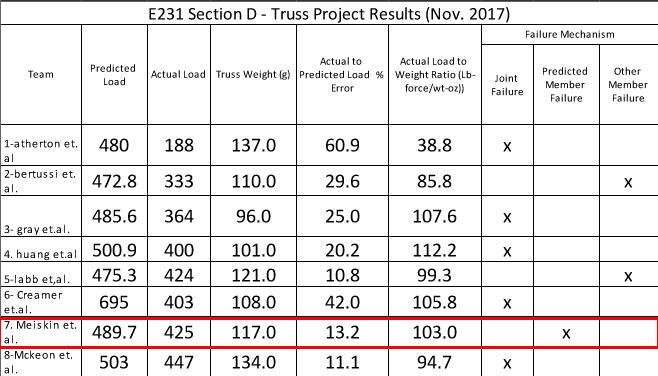
\includegraphics[height=8cm]{TrussResults.png}}\end{center}

\subsection{Figure 16: Truss Failure}
\begin{center}{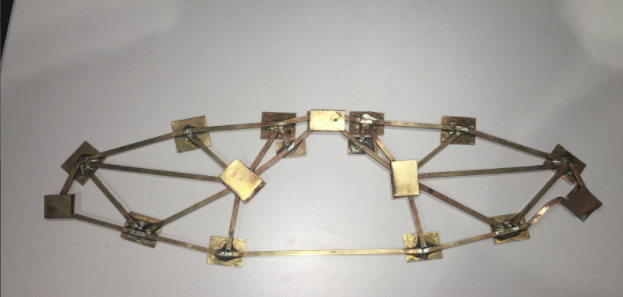
\includegraphics[height=8cm]{BuckledTruss.png}}\end{center}

\subsection{Figure 17: Joint Failure}
\begin{center}{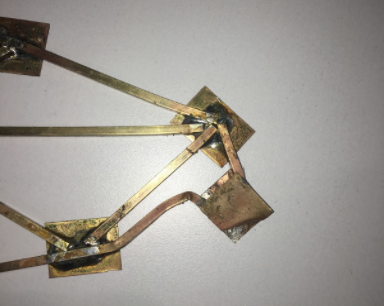
\includegraphics[height=8cm]{BuckledMember.png}}\end{center}

\end{document}
